\documentclass{beamer}

\mode<presentation>
{
    %\usetheme{Warsaw}
    \definecolor{links}{HTML}{2A1B81}
    \hypersetup{colorlinks,linkcolor=,urlcolor=links}
    \usetheme{Frankfurt}
    %\usecolortheme{seagull}
    % or ...
    \setbeamercovered{transparent}
    % or whatever (possibly just delete it)
}

\usepackage[english]{babel}
\usepackage[utf8]{inputenc}
\usepackage{times}
\usepackage[T1]{fontenc}
\usepackage{fancyvrb}
\usepackage{listings}
\usepackage{graphicx}
\usepackage{attachfile}
\usepackage{ifthen}

\newboolean{localPieces} %Declaration, defaults to false
\setboolean{localPieces}{false} %Assignment

\title{Advanced Csound}

\author[Gogins] % (optional, use only with lots of authors)
{Michael Gogins \\ \url{http://michaelgogins.tumblr.com} }
% - Give the names in the same order as the appear in the paper.
% - Use the \inst{?} command only if the authors have different
%   affiliation.

\institute[Irreducible Productions] % (optional, but mostly needed)
{
    Irreducible Productions\\
    New York
}
% - Use the \inst command only if there are several affiliations.
% - Keep it simple, no one is interested in your street address.

\date[NYCEMF 2022] % (optional, should be abbreviation of conference name)
{NYCEMF 2022}
% - Either use conference name or its abbreviation.
% - Not really informative to the audience, more for people (including
%   yourself) who are reading the slides online

\subject{Computer Music}
\expandafter\def\expandafter\insertshorttitle\expandafter{%
    \insertshorttitle\hfill%
    \insertframenumber\,/\,\inserttotalframenumber}
% This is only inserted into the PDF information catalog. Can be left
% out. 
\begin{document}
    \lstset{basicstyle=\ttfamily\tiny,commentstyle=\ttfamily\tiny,tabsize=2,breaklines,fontadjust=true,keepspaces=false,fancyvrb=true,showstringspaces=false,moredelim=[is][\textbf]{\\emph\{}{\}}}
    
    \begin{frame}
        \titlepage
    \end{frame}
    
    \begin{frame}{Outline I}
        \begin{itemize}
            \item These are slides, with links to resources, for a workshop on the
            \textit{advanced} use of Csound.
            \item The intended audience is anyone using Csound to \textit{actually make
                music}, whether they are a raw beginner or an experienced user.           
             \item \textit{There are no compromises here}, but I will try to keep things
            as simple as possible.
        \end{itemize}
    \end{frame}
    
    \begin{frame}{Outline II}
        \begin{itemize}
           \item First we review "best practices" using \textit{built-in features of
            the current release of Csound}.
            \item I also introduce a number of extensions to Csound: 
                \begin{itemize}
                    \item Development environments.
                    \item Plugin opcodes.
                    \item Hosting VST plugins.
                    \item Using other languages in Csound.
                \end{itemize}
        \end{itemize}
    \end{frame}
    
    \begin{frame}{Basic Pre-Requisites}
    	Install with brew on macOS, apt on Linux, vcpkg on Windows, or 
	google for downloads.
        \begin{itemize}
            \item This workshop uses the basic but quite cross-platform text editor \texttt{gedit} 
            for both writing and running Csound pieces.
            \item Install the latest Csound for your desktop from
            \url{https://csound.com/download.html}. For the current release on
            Linux, build Csound from sources 
            (\url{https://github.com/csound/csound/blob/develop/BUILD.md}).
            \item CsoundWebAudio is included in workshop materials but can be 
            downloaded from \url{https://github.com/gogins/csound-extended-wasm/releases}.
            \item Install the Audacity soundfile editor for your desktop from
            \url{https://www.audacityteam.org/download/}.
        \end{itemize}
    \end{frame}
    
    \begin{frame}{Optional Pre-Requisites}
        Many of these have their own additional pre-requisites. 
        \begin{itemize}
            \item ABX comparator from \url{https://github.com/gogins/python-abx}.
            \item Python 3.9 from \url{https://www.python.org/downloads/}.
            \item Faust DSP language from
            \url{https://github.com/grame-cncm/faust/releases}.
            \item Csound plugin opcodes from
            \url{https://github.com/csound/plugins}, needs to be built from sources.
        \end{itemize}
    \end{frame}
    
    \begin{frame}{Agenda}
        \tableofcontents
        % You might wish to add the option [pausesections]
    \end{frame}
    
    \section{Hearing Electroacoustically}
    
    \begin{frame}{Hearing}
    	\begin{itemize}
	  \item Before anything else one should know that one is hearing \textit{objectively}.
	  \item One should establish the limits of one's hearing because the computer 
	  will exceed them.
	  \item One should establish the least noticeable differences for important features of sound. 
	\end{itemize}
    \end{frame}
    \begin{frame}{Exercise: Hearing}
    	\begin{itemize}
	  \item Ideally get a hearing test from an audiologist.
	  \item Frequency sweep in Audacity.
	  \item Dynamic ranges in Audacity.
	  \item Wave table sizes in Audacity.
	  \item Time/frequency uncertainty relation.
	  \item Digital artifacts in Audacity: clicking, aliasing, smearing.
	\end{itemize}
    \end{frame}
    
    \section{Introduction to Csound}
    \begin{frame}{Csound}
        \begin{itemize}
            \item Csound is a \textit{programmable} software sound synthesizer.
            \item Csound dates from 1985, yet is still being developed (with almost
            complete backward compatibility).
            \item All SWSS have digital oscillators, filters, envelopes, etc...
            \textit{because} it is older, Csound has \textit{more} unit generators.
            \item Csound can be extended with plugins, some of which bring other
            programming languages into Csound. 
            \item Csound has a flexible API, and can be embedded in many other
            programming languages.
            \item Csound began with "off-line rendering," but now does real-time
            audio and interactive performance very well.
            \item Csound runs on desktops, mobile devices, and Web
            browsers. Here, we focus on desktops and browsers.
        \end{itemize}
    \end{frame}
    \begin{frame}{An "All-In" Piece}
        \begin{itemize}
            \item Here I will perform a real-time, interactive, algorithmic piece
            that uses much of what we will work with today.
            \item This piece is one .html file that incorporates  HTML, JavaScript, and Csound.
            \item But it is still just one .html file that is edited in a code editor
            like any other code, and that runs in one process like any other program.
        \end{itemize}
    \end{frame}
    
    \section{Coding for Csound}
    
    \begin{frame}{The Playpen Concept}
        \begin{itemize}
            \item A "playpen" is where you can play with things and not worry 
            about breaking them.
            \item In computer music we have an iterative work cycle:
            	\begin{itemize}
		   \item \textit{Edit} a piece.
		   \item \textit{Compile} the piece. If it doesn't compile, go back to \textit{Edit}.
		   \item \textit{Run} the piece to render audio. If it doesn't run, go back to \emph{Edit}.
		   \item \textit{Listen} to the piece. If you don't like it, go back to \emph{Edit}.
		   \item When you don't need to go back to \emph{Edit}, the piece is done.
	        \end{itemize}
            \item  We will make a playpen that makes these steps as fast and 
            automatic as possible, so that we can concentrate on making music.
            \item We can make our playpen by customizing a code editor, or by 
            using a code editor specifically designed for Csound.
          \end{itemize}    
    \end{frame}
    
    \begin{frame}{Code Editors}
        \begin{itemize}
            \item A Csound piece consists of one or more source code files that are
            edited in a code editor and translated to sound by a runtime compiler, which is
            Csound.
            \item Unlike other SWSS such as SuperCollider or Max, Csound does not
            come with its own visual patcher or a graphical user interface "front end."
            \item Nevertheless using a code editor or a dedicated "front end"
            program can make the user significantly more productive.
            \item This workshop uses gedit with external commands as a front end, but you 
            may find other editors more useful.
        \end{itemize}
    \end{frame}
    
    \begin{frame}{Code Editors for Csound}
        \begin{itemize}
            \item blue from \url{https://blue.kunstmusik.com/}.
            \item CsoundQt from \url{http://csoundqt.github.io/}.
            \item Cabbage from \url{https://www.cabbageaudio.com/}.
            \item Visual Studio Code from \url{https://code.visualstudio.com/} with
            Csound extension from \url{https://github.com/csound/csound-vscode-plugin}.
        \end{itemize}
    \end{frame}
    
    \begin{frame}{Configuring the Csound Environment}
    	\begin{itemize}
		\item The \texttt{csound} program should be in your environment's \texttt{PATH} variable.
		\item For the \texttt{vst4cs opcodes}, we configure Csound to load them from their build or download directories.
		\item For the Csound plugins repository, we build them locally and install using \texttt{sudo make install}.
		\item Shown for macOS, but the same variables should be set with appropriate values on Linux or Windows.
	\end{itemize}
    \end{frame}    
    \begin{lstlisting}
export OPCODE6DIR64="/Users/michaelgogins/Downloads"
export RAWWAVE_PATH="/opt/homebrew/Cellar/stk/4.6.2/share/stk/rawwaves"
     \end{lstlisting}
    
    \begin{frame}{Coding for High-Quality Audio}
        \begin{itemize}
            \item Many of Csound's opcodes, man pages, and examples are old, and
            prioritize memory and run time over audio quality.
            \item \textit{Today, prioritize audio quality in all cases}.
            \item Use a sample rate of 48,000 or even 96,000 frames per second with
            \texttt{ksmps = 100} or even \texttt{ksmps = 1}.
            \item Use the double-precision version of Csound (now default).
            \item Render to floating-point soundfiles for high dynamic range.
            \item Use table sizes of at least 65,537 for lower noise.
            \item Use \textit{audio-rate} envelopes.
            \item Use the \textit{latest versions} of opcodes.
            \item Used in this way, Csound competes on audio quality with
            \textit{any} open source or commercial software.
        \end{itemize}
    \end{frame}
    
    \begin{frame}{Exercise: Coding for High-Quality Audio}
        \begin{itemize}
            \item Run the original version of \textit{\textbf{Xanadu}} in your code
            editor, listen on headphones, and examine the spectrogram in Audacity.
            \item Run the high-resolution version of \textit{\textbf{Xanadu}} in
            your code editor, listen on headphones, and examine the spectrogram in Audacity.
        \end{itemize}
    \end{frame}
    
    \begin{frame}{Software Design}
        \begin{itemize}
            \item \textbf{Encapsulation} Hide functionality in \textit{modules} that
            expose only inputs and outputs. Define modules with \texttt{instr} and
            \texttt{opcode}, corresponding to classes and functions.
            \item \textbf{Abstraction} Define abstract interfaces for instruments or
            UDOs that perform similar functions; e.g. different synths should use the same
            pfields.
            \item \textbf{Normalization} Use \textit{musical} units: MIDI key not
            Hz, MIDI velocity not amplitude.
            \item \textbf{Signal Flow} Signals flow from input devices through
            opcodes to instruments; from opcode to opcode through variables; from
            instruments through opcodes to output devices. Processing is first by
            instrument number, then by order of definition. Signals also flow through
            control channels and global variables.
        \end{itemize}
    \end{frame}
    
    \begin{frame}{Modular Design}
        \begin{itemize}
            \item Using naming conventions to simulate namespaces.
            \item Normalize pfields and variables.
            \item Associate global function tables with modules.
            \item Associate global control variables with modules, and use
            \texttt{chnexport} to  export these variables as control channels.
            \item Define signal flow in the orchestra header, \textit{not} inside modules.
        \end{itemize}
    \end{frame}
    
    \begin{frame}{Exercise: MIDI Interop}
    	\begin{itemize}
		\item \texttt{insdef\_score.csd} uses an instrument definition designed to be driven by a Csound score.
		\item \texttt{insdef\_midi.csd}  uses a similar instrument definition designed to be driven by a MIDI controller (or MIDI file).
		\item \texttt{insdef\_interop.csd}  modifies the instrument definition to work equally well in all these ways.
		\item \texttt{insdef\_interop.html} shows how to use this instrument with the trigger-release model used by modular analog synthesizers.
	\end{itemize}
    \end{frame}
    
    \section{Useful Builtin Opcodes}
    
    \begin{frame}{A Modular Design for Spatialization I}
        \begin{itemize}
            \item Modules are big rectangles. Some are instruments, some are user-defined opcodes, some are built-in opcodes.
            \item Inputs are small rectangles on the tops of modules.
            \item Outputs are small rectangles on the bottoms of modules.
            \item Signals flow from inputs to modules, from modules to outputs, and from outputs to inputs.
            \item We will use user-defined opcodes to add motion cues (doppler effect) and distance cues (lowpass by distance) to Csound's builtin spatialization opcodes.
            \item \textit{\textbf{Note:}} Modules can be nested inside other modules; this is exactly what makes code easier to design and to understand.
        \end{itemize}
    \end{frame}

    \begin{frame}{A Modular Design for Spatialization II}
        \begin{figure}
            \centerline{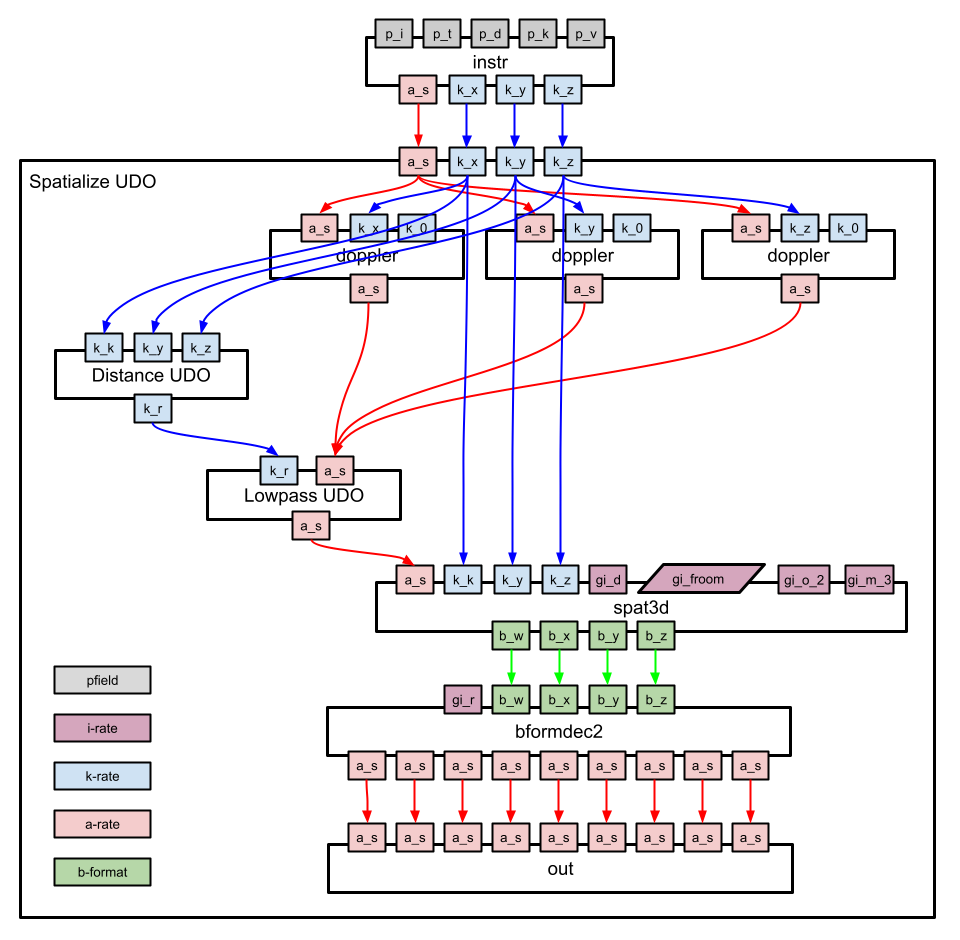
\includegraphics[height = 0.66\textwidth]{Spatialization}}
        \end{figure}        
    \end{frame}
    
    \begin{frame}{A Modular Design for Spatialization III}
        \begin{itemize}
            \item \texttt{spat3d} spatializes a sound in a user-defined "room" using Ambisonic panning, wall reflections, and interpolated movement. It's not bad. 
            \item \texttt{bformdec2} decodes an Ambisonic signal to various speaker setups or "rigs." It's pretty good.
            \item We put these opcodes into a handy module, a UDO.
            \item This is not enough. Real spatialization involves Doppler effects and fading higher frequencies with distance.
            \item There must be one Doppler calculation for each independent dimension of motion, so we put 3 \texttt{doppler} opcodes into our UDO and average them.
            \item Similarly we put in a \texttt{lopass2} opcode and adjust the cutoff by distance from the listener.
            \item The dopplered and filtered sound goes to \texttt{spat3d}, then to \texttt{bformdec2}, then to Csound's audio output.
        \end{itemize}
    \end{frame}

    \begin{frame}{Exercise: Spatializing a Flock}
        \begin{itemize}
            \item A flock of N notes from M instruments, moving in {time, pitch,
                space}.
            \item Spatialize the voices moving.
        \end{itemize}
    \end{frame}
    
    \begin{frame}{Streaming Phase Vocoder}
        \begin{itemize}
            \item The PVS opcodes are a modular toolkit for time/frequency analysis, processing, and resynthesis, either in real time or off-line.
            \item The PVS opcodes use \texttt{fsig} variables that carry either amplitude/frequency data (from FFT analysis), or amplitude/frequency/phase/track ID (partial track) data (more suited to processing).
            \item Other SWSS have similar facilities, but Csound's PVS opcodes are more complete and more orthogonal.
            \item Csound has several \textit{other} facilities for time/frequency processing!
        \end{itemize}
    \end{frame}
        
        \begin{frame}{Exercise: Processing Microphone Input}
        \end{frame}
        
        \section{Useful Plugin Opcodes}
        \subsection{Faust Language for DSP}
        \subsection{FluidSynth}
        \subsection{Opcodes for External Plugins}
        \section{Using Other Languages with Csound}
        \subsection{Python}
        \subsection{C++}
        \subsection{HTML/JavaScript}
        
        \begin{frame}[allowframebreaks]
            \frametitle<presentation>{References}
            
            \begin{thebibliography}{10}
                
                \beamertemplatebookbibitems
                % Start with overview books.
                
                \bibitem{GBlog} \href{http://michaelgogins.tumblr.com/}{Michael Gogins, blog}.
                
                \bibitem{GGithub} \href{https://github.com/gogins/gogins.github.io}{Michael
                    Gogins. ``Computer Music Resources.''}
                
                \bibitem{CQT2008}
                \href{http://www.sciencemag.org/content/320/5874/346.abstract}{Clifton
                    Callender, Ian Quinn, and Dmitri Tymoczko. ``Generalized voice-leading spaces.''
                    \emph{Science}, 320:346–
                    348, 2008.}
                
                \bibitem{G1991} {Michael Gogins. ``How I Became Obsessed with Finding a
                    Mandelbrot Set for Sounds,'' \textbf{\textit{News of Music}}
                    \textbf{13}:129-139.}
                
                \bibitem{FS2005}
                \href{http://www.mtosmt.org/issues/mto.05.11.3/mto.05.11.3.fiore_satyendra.pdf}{T.M.
                    Fiore and R. Satyendra. ``Generalized Contextual
                    Groups.'' \emph{Music Theory Online}, 11(3), 2005}.
                
                \bibitem{G2006}
                
                \href{https://www.dropbox.com/s/ztej71n2fbn4tq4/Lindenmayer_Systems_Based_on_Riemannian_Transformations.pdf}{Michael
                    Gogins. ``Score generation in voice-leading
                    and chord spaces.'' In Georg Essl and Ichiro Fujinaga,
                    editors, \emph{Proceedings of the 2006 International Computer Music Conference},
                    San Francisco, California,
                    2006. International Computer Music Association.}
                
                \bibitem{T2006}
                \href{http://www.sciencemag.org/content/313/5783/72.abstract?ijkey=wzKBea3ktKdu2&keytype=ref&siteid=sci}{Dmitri
                    Tymoczko. ``The Geometry of Musical Chords.'' \emph{Science}, 313:72–74, 2006.}
                
            \end{thebibliography}
            
        \end{frame}
        
    \end{document}
    
    
    
